 

\section{Введение}

В данной лабораторной работе проводится измерение сопротивления резисторов с помощью универсального моста E7-4. Цель работы заключается в освоении методики использования измерительного прибора для многократного прямого измерения физической величины, а также в выполнении простейшей статистической обработки серии результатов наблюдений при прямых измерениях.

Измерение сопротивления является одной из базовых задач в физическом эксперименте, так как сопротивление является важной характеристикой электрических цепей и компонентов. Для точного измерения сопротивления используется мостовая схема, которая позволяет с высокой точностью определить значение сопротивления путем сравнения с известными эталонными значениями.

В ходе работы предстоит изучить принцип работы универсального моста E7-4, освоить методику измерения сопротивления, а также провести многократные измерения для получения серии результатов. Полученные данные будут подвергнуты статистической обработке, включая построение гистограммы и графика распределения результатов, что позволит оценить случайные погрешности измерений и определить среднее значение сопротивления с учетом погрешности.

\subsection{Цель работы}

\begin{enumerate}
\item
    Освоить методику использования измерительного прибора для 
многократного прямого измерения физической величины. 
\item
Выполнить простейшую статистическую обработку серии вычислений.
\end{enumerate}
\subsection{Решаемые задачи}

В лабораторной работе №1в решаются задачи по освоению методики использования универсального моста E7-4 для измерения сопротивления резисторов. Проводится серия многократных измерений с использованием грубой и точной шкал прибора, результаты которых фиксируются для последующей статистической обработки.

\section{Основная часть}

\subsection{Теоретическая часть}
Формула относительной погрешности прибора $\delta R$:
\begin{equation}
    \delta R = \pm\left(1+\frac{R}{6}\right)
\end{equation}
Где $R$ - показания прибора. 
Формула для нахождения среднего арифметического $\bar{R}$:
\begin{equation}
    \bar{R}=\frac{\sum_{i=1}^{n} R_i}{n}
\end{equation}
Здесь $n$ - количество результатов наблюдений, $R_i$ - результат измерения отдельного наблюдения.
Расчёт погрешности прибора $\Delta R$ вычисляется ледующим образом:
\begin{equation}
    \Delta R = \frac{\delta R\cdot\bar{R}}{100\%}
\end{equation}
Среднеквадратичное отклонение $\sigma$:
\begin{equation}
    \sigma \approx \sqrt{\frac{1}{n-1}\sum_{i=1}^{n} (R_i-\bar{R})^2}
\end{equation}
Средняя квадратичная погрешность среднего $\Delta R$:
\begin{equation}
    \Delta R={\sigma}_{\bar{R}}\approx\frac{\sigma}{\sqrt{n}}
\end{equation}

\subsection{Эксперимент}
Подготовка к эксперименту начинается с изучения описаний и правил пользования приборами, которые будут использоваться в работе, в частности, универсального моста E7-4. Перед началом измерений необходимо собрать установку по рекомендуемой блок-схеме (рис. 1), подключив измеряемое сопротивление $R$ к зажимам «С—L—R» моста. Установка переключателя «С, L, ~R, =R» зависит от типа измеряемого тока (постоянный или переменный), а ручка переключателя «ЧАСТОТА Hz» устанавливается в положение «100» (для переменного тока) или «1000» (для постоянного тока). Чувствительность индикатора настраивается так, чтобы стрелка прибора находилась в пределах 2/3 шкалы, а с помощью ручки «МНОЖИТЕЛЬ» добиваются минимального показания прибора. После этого мост уравновешивается, регулируя чувствительность и используя ручки «ОТСЧЁТ», чтобы добиться наименьшего показания на индикаторе равновесия. Измеренное сопротивление рассчитывается как сумма отсчетов по шкалам переключателя и потенциометра «ОТСЧЁТ», умноженная на соответствующий множитель.
\newline
Выполнение эксперимента включает несколько этапов. Сначала измеряется заданное значение сопротивления несколько раз (10 измерений) на грубой шкале прибора, результаты записываются в таблицу для анализа проявления случайных погрешностей. Затем выбирается более чувствительная шкала, и проводятся 50 или более измерений для формирования выборки, подлежащей статистической обработке. Результаты этих измерений также фиксируются в таблице, включая случайные отклонения от среднего значения и их квадраты. После завершения измерений прибор переключается на самую грубую шкалу, установка сдается лаборанту, и электрическая цепь разбирается.



\begin{figure}[ht!]
\centering
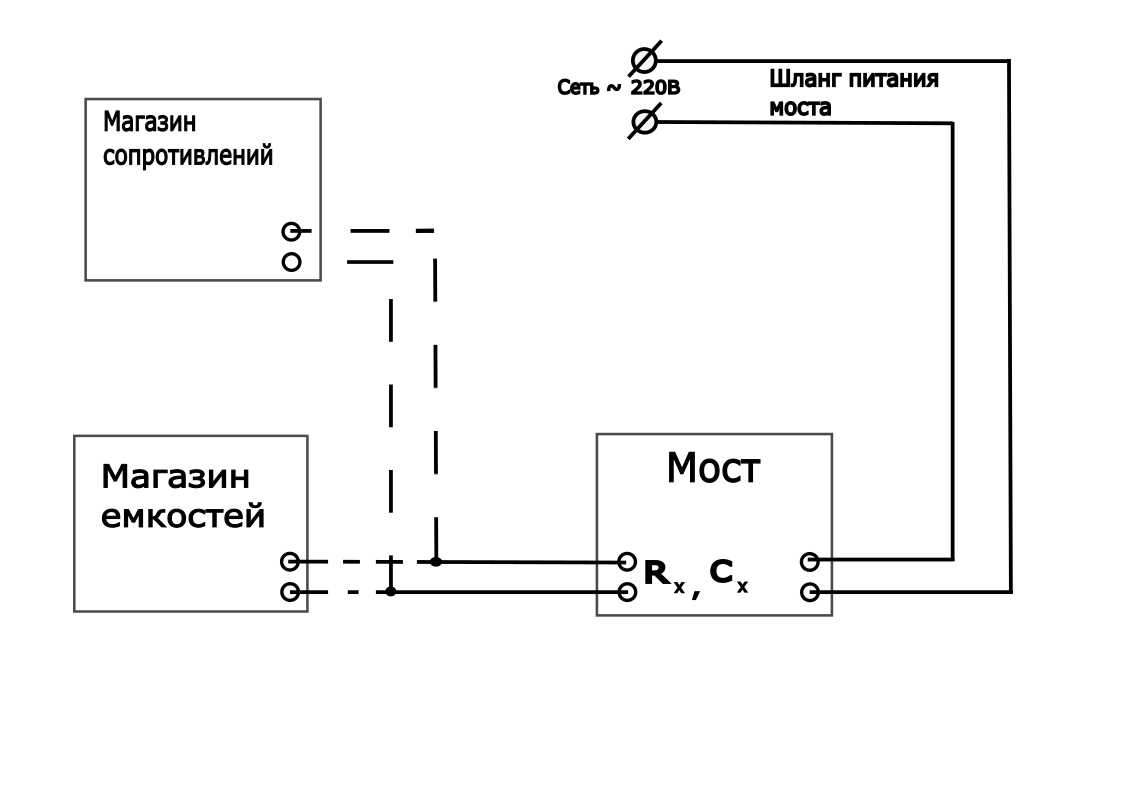
\includegraphics[width=0.8\textwidth]{схема}
\caption{схема моста Е7-4}
\label{fig:sketch}
\end{figure}

\begin{figure}[ht!]
\centering
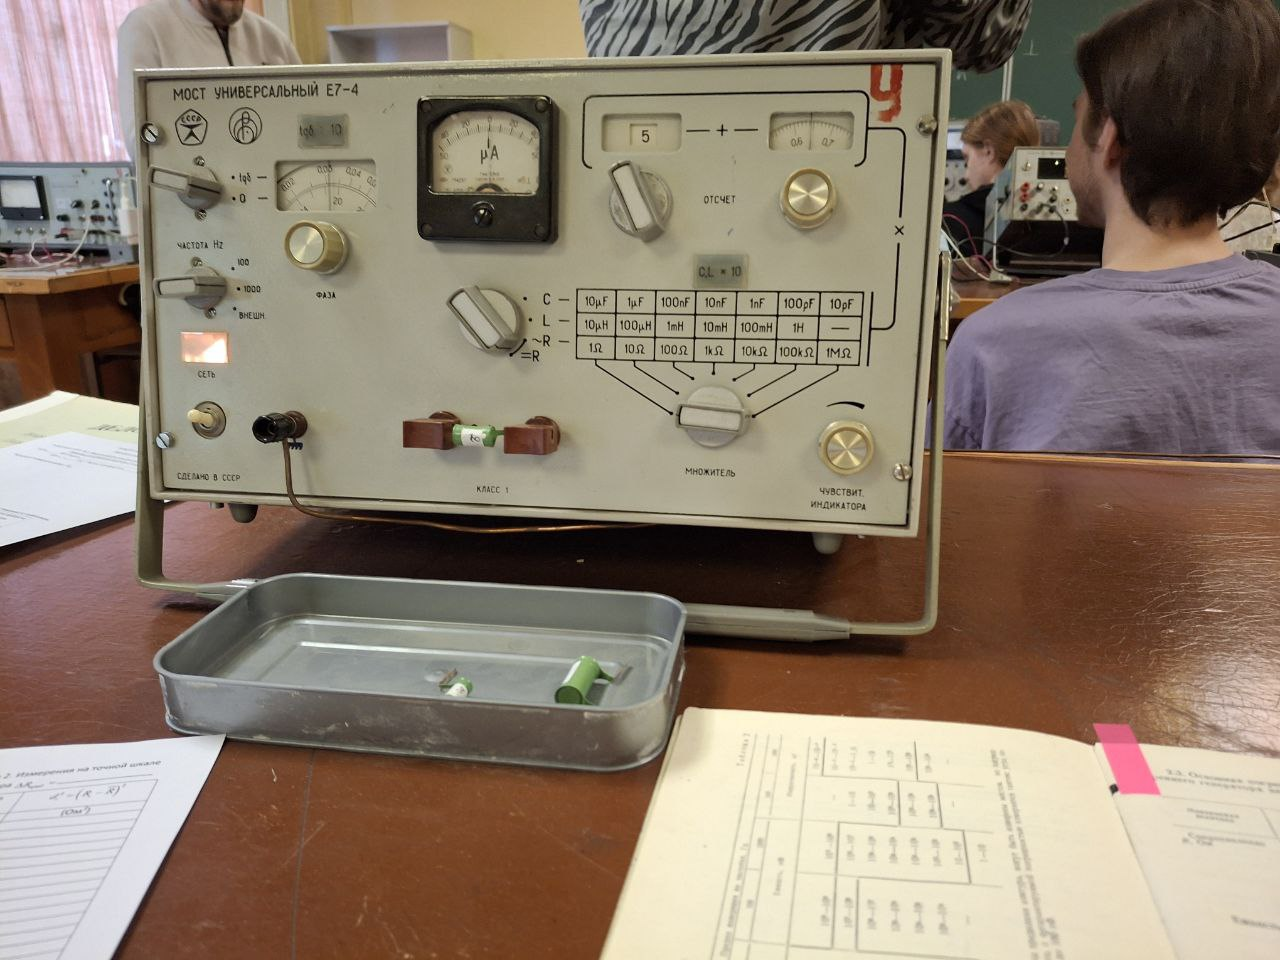
\includegraphics[width=0.8\textwidth]{device}
\caption{Мост Е7-4}
\label{fig:device}
\end{figure}
\newpage
\subsection{Обработка данных и обсуждение результатов}
Описываются методы обработки данных, освещаются особенности реализованных алгоритмов.

\subsubsection{Исходный код}
Для написания программы, вычисляющей все требуемые данные, использу
ется язык $C++$; среда разработки- $Visual Studio$.
 Код разбит на несколько файлов: main.cpp, DataProc.cpp, DataProc.h.
 В файле DataProc.h объявлены все используемые библиотеки и функции, которые реализует программа, в Файле DataProc.cpp находятся определения функций: функция нахождения среднего арифметического, функция нахождения всех случайных отклонений из данной выборки, функция нахождения стандартных отклонений и т.д. 
 Файл main.cpp отвечает за вывод данных в файл .tex в формате таблицы.
 Ниже представлены реализации функций считывания данных из файла (см. Листинг 1), поиска среднего квадратичного отклонения $\sigma$ и средней квадратичной погрешности среднего $\Delta R$ соответственно.
\newpage
\begin{lstlisting}[label=listing1, caption=Считывание данных их файла]
#include<iostream>

void DataProcessor::readData() {
    std::ifstream inputFile(inputFileName);
    if (!inputFile.is_open()) {
        throw std::runtime_error("Не удалось открыть файл");
    }
    double value;
    while (inputFile >> value) {
        data.push_back(value);
    }
    inputFile.close();
}
\end{lstlisting}

Поиск среднего квадратичного отклонения $\sigma$:
\begin{verbatim}
void DataProcessor::calculateStandardDeviation() {
    double sumSquaredDeviations = 0.0;
    for (double squaredDev : squaredDeviations) {
        sumSquaredDeviations += squaredDev;
    }
    standardDeviation = std::sqrt(sumSquaredDeviations / data.size());
}
\end{verbatim}
Поиск средней квадратичной погрешности среднего $\Delta R$:
\begin{verbatim}
    void DataProcessor::calculateMeanError() {
    meanError = standardDeviation / std::sqrt(data.size());
}
\end{verbatim}
\newpage
\subsubsection{Таблицы}

\begin{center}
\begin{table}[h!]
\centering
\caption{Результаты грубых измерений}
\label{tabl:1}
\begin{tabular}{|c|c|c|c|c|}
\hline
\begin{minipage}{7mm}
    № п.п. 
\end{minipage}&
\begin{minipage}{5cm}
    Диапазон показаний использованной шкалы прибора
\end{minipage} &
\begin{minipage}{5cm}
    Результаты отдельных наблюдений ($R_i$)
\end{minipage} &
\begin{minipage}{5cm}
    Погрешность прибора на данной шкале ($\Delta R_{\text{приб}}$)
\end{minipage}\\
\hline
{}&Ом&Ом&Ом\\
\hline
1 &	0-10  &	6 & 0.12 \\
2 &	0-10  &	6	& 0.12 \\
3 &	0-10  &	6	& 0.12 \\
4 &	0-10  &	6 & 0.12 \\
5 & 0-10  &	6 & 0.12 \\
6 & 0-10  &	6 & 0.12 \\
7 & 0-10  &	6 & 0.12 \\
8 & 0-10  &	6 & 0.12 \\
9 & 0-10  &	6 & 0.12 \\
10& 0-10  &	6 & 0.12 \\
\hline
\end{tabular}
\end{table}
\end{center}

\begin{longtable}{|c|c|c|c|}
\caption{Измерения на точной шкале}
\label{tabl:2}
\hline
\begin{minipage}{7mm}
    № п.п. 
\end{minipage}&
\begin{minipage}{5cm}
    Диапазон показаний использованной шкалы прибора
\end{minipage} &
\begin{minipage}{5cm}
    Результаты отдельных наблюдений ($R_i$)
\end{minipage} &
\begin{minipage}{5cm}
    Погрешность прибора на данной шкале ($\Delta R_{\text{приб}}$)
\end{minipage}\\
\hline
{}&Ом&Ом&Ом\\
\hline
1 & 5,93 & -0.0104 & 0.000108 \\  
2 & 5,95 & 0.0096 & 9.216e-05 \\  
3 & 5,95 & 0.0096 & 9.216e-05 \\  
4 & 5,94 & -0.0004 & 1.6e-07 \\  
5 & 5,93 & -0.0104 & 0.000108 \\  
6 & 5,94 & -0.0004 & 1.6e-07 \\  
7 & 5,94 & -0.0004 & 1.6e-07 \\  
8 & 5,95 & 0.0096 & 9.216e-05 \\  
9 & 5,95 & 0.0096 & 9.216e-05 \\  
10 & 5,93 & -0.0104 & 0.000108 \\  
11 & 5,94 & -0.0004 & 1.6e-07 \\  
12 & 5,95 & 0.0096 & 9.216e-05 \\  
13 & 5,94 & -0.0004 & 1.6e-07 \\  
14 & 5,93 & -0.0104 & 0.000108 \\  
15 & 5,95 & 0.0096 & 9.216e-05 \\  
16 & 5,95 & 0.0096 & 9.216e-05 \\  
17 & 5,94 & -0.0004 & 1.6e-07 \\  
18 & 5,95 & 0.0096 & 9.216e-05 \\  
19 & 5,93 & -0.0104 & 0.000108 \\  
20 & 5,94 & -0.0004 & 1.6e-07 \\  
21 & 5,95 & 0.0096 & 9.216e-05 \\  
22 & 5,94 & -0.0004 & 1.6e-07 \\  
23 & 5,95 & 0.0096 & 9.216e-05 \\  
24 & 5,95 & 0.0096 & 9.216e-05 \\  
25 & 5,93 & -0.0104 & 0.000108 \\  
26 & 5,93 & -0.0104 & 0.000108 \\  
27 & 5,95 & 0.0096 & 9.216e-05 \\  
28 & 5,95 & 0.0096 & 9.216e-05 \\  
29 & 5,94 & -0.0004 & 1.6e-07 \\  
30 & 5,93 & -0.0104 & 0.000108 \\  
31 & 5,94 & -0.0004 & 1.6e-07 \\  
32 & 5,93 & -0.0104 & 0.000108 \\  
33 & 5,94 & -0.0004 & 1.6e-07 \\  
34 & 5,95 & 0.0096 & 9.216e-05 \\  
35 & 5,93 & -0.0104 & 0.000108 \\  
36 & 5,94 & -0.0004 & 1.6e-07 \\  
37 & 5,93 & -0.0104 & 0.000108 \\  
38 & 5,95 & 0.0096 & 9.216e-05 \\  
39 & 5,94 & -0.0004 & 1.6e-07 \\  
40 & 5,94 & -0.0004 & 1.6e-07 \\  
41 & 5,94 & -0.0004 & 1.6e-07 \\  
42 & 5,93 & -0.0104 & 0.000108 \\  
43 & 5,94 & -0.0004 & 1.6e-07 \\  
44 & 5,95 & 0.0096 & 9.216e-05 \\  
45 & 5,93 & -0.0104 & 0.000108 \\  
46 & 5,94 & -0.0004 & 1.6e-07 \\  
47 & 5,93 & -0.0104 & 0.000108 \\  
48 & 5,94 & -0.0004 & 1.6e-07 \\  
49 & 5,94 & -0.0004 & 1.6e-07 \\  
50 & 5,94 & -0.0004 & 1.6e-07 \\  
\hline
\end{longtable}



\newpage
\begin{table}[h!]
\centering
\caption{Распределение результатов измерений}
\label{tab:distribution}
\begin{tabular}{|c|c|c|c|}
\hline
\begin{minipage}{7mm}
    № п.п. 
\end{minipage}&
\begin{minipage}{5cm}
    Границы интервалов (ширина интервала 0.01 Ом)
\end{minipage} &
\begin{minipage}{5cm}
    Число случаев ($\Delta n$), когда результат наблюдения попадает в данный интервал
\end{minipage} &
\begin{minipage}{5cm}
    Доля полного числа результатов, попадающих в данный интервал ($\delta n = \frac{\Delta n}{n}$)
\end{minipage}\\
\hline
1    & 5.90    & 0    & 0.00   \\
2    & 5.91   & 0   & 0.00    \\
3    & 5.92    & 0    & 0.00    \\
4    & 5.93    & 14   & 0.28    \\
5    & 5.94    & 20    & 0.4    \\
6    & 5.95    & 16    & 0.32    \\
7    & 5.96    & 0    & 0.00    \\
8    & 5.97    & 0    & 0.00    \\
9    & 5.98    & 0    & 0.00    \\
10   & 5.99    & 0    & 0.00    \\
11   & 6.0   & 0    & 0.00    \\
\hline
\end{tabular}
\end{table}

\newpage

\subsubsection{Графики}


\begin{figure}[ht!]
\centering
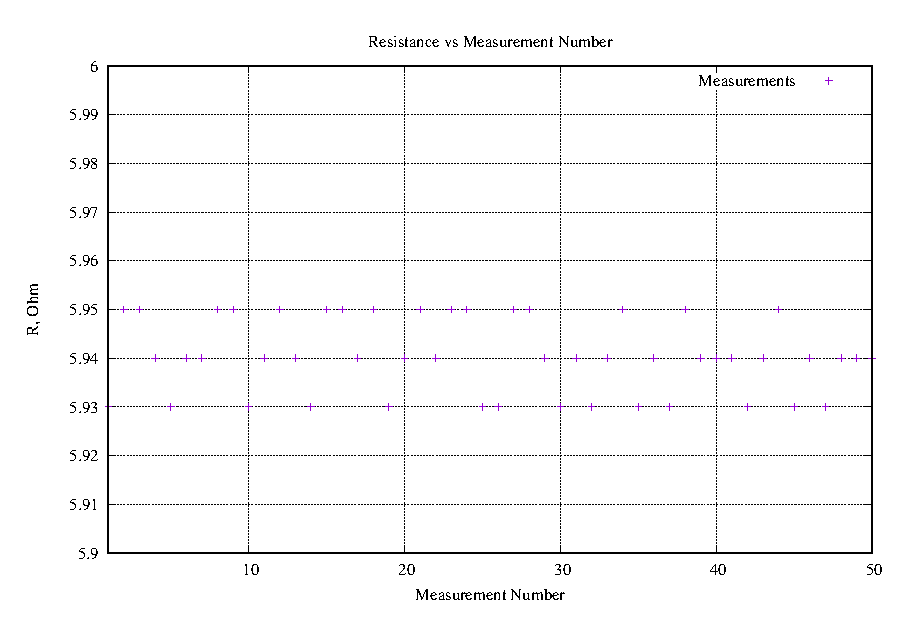
\includegraphics[width=0.8\textwidth]{resistance_plot}
\caption{Зависимость результатов измерения от времени}
\label{fig:plot}
\end{figure}

\begin{figure}[ht!]
\centering
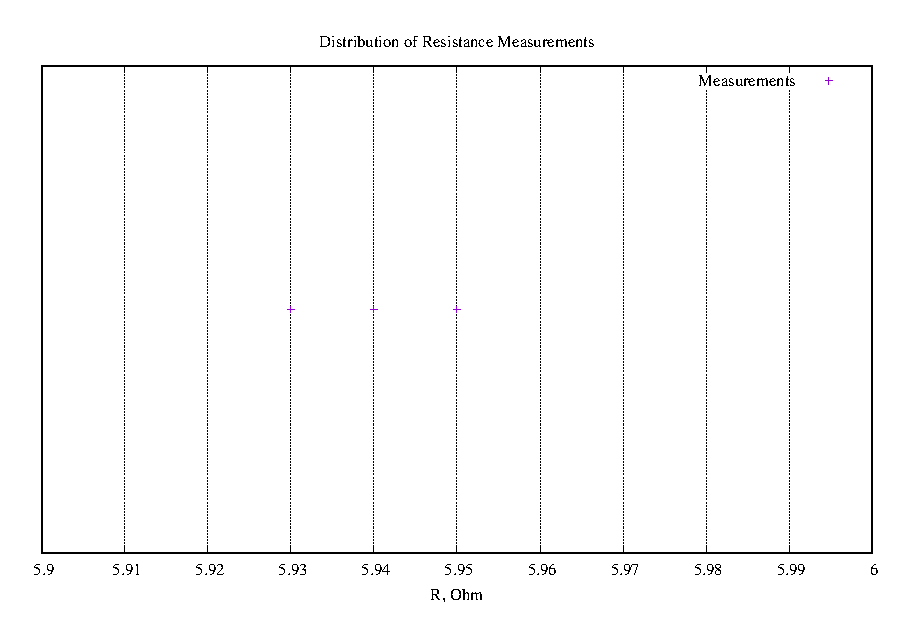
\includegraphics[width=0.8\textwidth]{resistance_distribution}
\caption{Значения измерений на числовой оси}
\label{fig:plot}
\end{figure}

\begin{figure}[ht!]
\centering
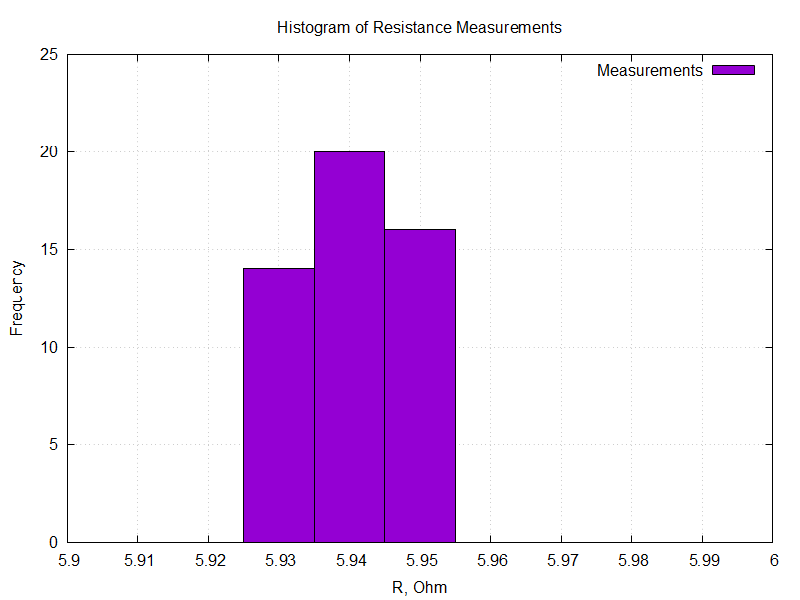
\includegraphics[width=0.8\textwidth]{resistance_histogram}
\caption{Гистограмма распределения}
\label{fig:plot}
\end{figure}
\newpage
\begin{figure}[ht!]
\centering
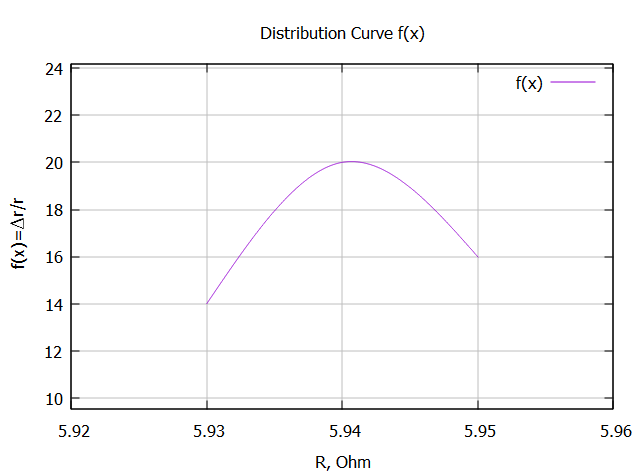
\includegraphics[width=0.8\textwidth]{distribution_curve}
\caption{График распределения}
\label{fig:plot}
\end{figure}

 \newpage


\section{Выводы}
В ходе выполнения лабораторной работы была освоена методика многократного прямого измерения сопротивления с использованием универсального моста E7-4. Работа позволила освоить навыки работы с измерительным прибором, научиться проводить статистическую обработку полученных данных и оценку случайных погрешностей.
Также были освоены базовые навыки работы с пакетами GNUplot и inkscape.

% Список литературы
% Для отчёта он не обязателен
\begin{thebibliography}{9}

%ссылка на репозиторий с исходныим кодом отчета и всех расчетных программ обязательна 
\bibitem{repo}
\url{https://github.com/st094830/labwork-1.git}  

\end{thebibliography}